\chapter{Methodology}
\section{Mini-Apps}
Mini-apps are a well established method of assessing new programming languages or techniques within HPC~\cite{Mallinson:2014, Slaughter:2015, martineau2017arch}. A mini-app is a small program which reproduces some functionality of a common HPC use case. Often, the program will be implemented using one particular technology, and then ported to another technology. The performance of the two mini-apps will then be tested, to see which technology is better suited to the particular problem represented by that mini-app. Such an approach gives quantitative data which provides a strong indication for the performance of a technology in a full implementation of an application. This dissertation will follow a similar approach of evaluating a program through the performance of a mini-app, using the test data to find any weaknesses in the Rust or original implementation.

I will also evaluate the ease with which I am able to port a mini-app into Rust. These observations will provide insight into what it is like to program in Rust, if its strict memory model and functional idioms help or hinder translation from the imperative languages which the ported programs are written in. This qualitative, partly experiential information will hopefully provide an insight into the actual practicalities of programming in Rust. For Rust to be fully accepted by the HPC community, it is necessary that the program fulfils the functional requirements of speed and scaling, alongside non functional requirements, of usability and user experience. The first factor provides a reason for using Rust programs in HPC, the second provides an impetus for learning how to write those programs.
\subsection{Selection}
So that a breadth of usage scenarios were examined, three mini-apps were selected based on their conformity to the following set of criteria.
\begin{itemize}
  \item \textbf{The program's kernel (i.e. the part of the program responsible for more than two thirds processing time) should not be more than 1500 lines.} To ensure that I fully implemented three ports of existing mini-apps, it was necessary to limit the size of the mini-apps that could be considered. This was an unfortunately necessary decision to make. Whilst it reduced the field of possible mini-apps, an analysis of the rejected mini-apps found that many of them devoted lots of code to subtle computational variations, which were of more importance to a particular rarefied domain, rather than presenting a novel approach to parallelism. (i could cite some benchmarks here like bookleaf or something)

  \item \textbf{The program must use shared memory parallelism and target the CPU.} Rust's (supposed) zero cost memory safety features are its unique feature. The best way to test the true cost of Rust's memory safety features would be through shared memory parallelism, where a poor implementation of memory management will make itself evident through poor performance. Programs which target the GPU rather than the CPU will not be considered, as the current implementations for Rust to target GPUs involve calling out to existing GPU APIs. Therefore, any analysis of a Rust program targeting a GPU would largely be an analysis of the GPU API itself.

  \item \textbf{The program run time should reasonably decrease as the number of threads increases, at least until the number of threads reaches 32.} It is important that any mini-app considered is capable of scaling to the high core counts normally seen in HPC.I will be running the mini-apps on Cirrus, which supports 36 real threads.

  \item \textbf{The program operate on data greater than the CPU's L3 Cache} so that we can be sure that the mini-app is representative of working on large data sets. Cirrus has an L3 cache of 45MiB. As each node has 256GB of RAM, a central constraint when working with large data sets is the speed with which data is loaded into the cache. Speed is often achieved by programs in this area through vectorisation, the use of which can be deduced from a program's assembly code. If there is a large performance difference between Rust and the reference mini-apps, we can use the program's assembly code to reason about that difference.

  \item \textbf{The program must be written in C or C++.} This restriction allows us to choose work which is more representative of HPC programs that actually run on HPC systems, rather than python programs which call out to pre-compiled libraries. Unlike Fortran, C and C++ use array indexing and layout conventions similar to Rust, which will make porting programs from them easier.

  \item \textbf{The program must use OMP.} This is a typical approach for shared memory parallelism in HPC. Use of a library to do the parallel processing also further standardises the candidate programs, which will lead to a deeper understanding between the mini-apps.
\end{itemize}

\subsection{Implementation}
Implementation of all three programs follows the same process, as outlined in Figure~\ref{fig:imp-flow}. Once a candidate mini-app is selected, it is implemented in Rust in serial. Any differences between the  behaviour of the Rust and the original implementation are thought of as bugs, and are eradicated or minimised as far as is possible. For ease of development, the Rust crate Clap was used to read command line arguments for the program, leading to Rust implementations of mini-apps being called with slightly different syntax. This difference was deemed to be so superficial as to be allowable. Program output was ensured to be as similar as possible to aid data-collection from both implementations.

\begin{figure}
  \center
  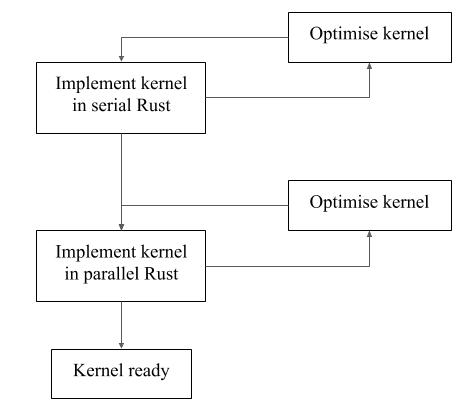
\includegraphics[height=12cm]{figs/ImplementationFlow.png}
  \caption{Flow Diagram for Implementation Process}
  \label{fig:imp-flow}
\end{figure}
\subsubsection{Babel Stream}

\section{Questionnaire}
